% !TEX encoding = UTF-8
% !TEX TS-program = pdflatex
% !TEX root = ../tesi.tex

\chapter{Fast-Broadcast}
	\label{chapter:fb}
	Fast-Broadcast \cite{4199282} is a multi-hop routing protocol for vehicular communication. Its main feature consists in breaking the assumption that all vehicles should know, \textit{a priori}, their fixed and constant transmission range. This assumption is often unreasonable, especially in \acrshort{vaneta}s and urban environments, where electromagnetic interferences and obstacles such as buildings heavily influence the transmission range.
	
	
	Fast-Broadcast employs two different phases:
	\begin{enumerate}
		\item the \textbf{Estimation Phase}, during which vehicles estimate their frontward and backward transmission range;
		\item the \textbf{Broadcast Phase}, during which a vehicle sends an Alert Message and the other cars need to forward it in order to propagate the information.
	\end{enumerate}

	\section{Estimation Phase}
		During this phase, vehicles try to estimate their frontward and backward transmission range by the means of Hello Messages. These beacons are sent periodically via broadcast to all the neighbors of a vehicle.
		
		
		Time is divided into turns and, in order to keep estimations fresh, data collected during a certain turn is kept for the duration of the next turn, then discarded. The parameter \textit{turnSize} specifies the duration of a turn: the authors suggest a duration of one second. A bigger \textit{turnSize} could guarantee less collisions to the detriment of freshness of information. On the other hand, the effects of a smaller \textit{turnSize} are specular to those just presented. 
		
		
		Using this approach, vehicles can estimate two different values:
		\begin{itemize}
			\item \textit{Current-turn Maximum Front Range (\textit{CMFR})}, which estimates the maximum frontward distance from which another car can be heard by the considered one;
			\item \textit{Current-turn Maximum Back Range} (\textit{CMBR}), which estimates the maximum backward distance at which the considered car can be heard.
		\end{itemize}
		When the turn expires, the value of these variables is stored in the \textit{LMFR} and \textit{LMBR} variables (\textit{Latest-turn Maximum Front Range} and \textit{Latest-turn Maximum Back Range}, respectively). The algorithm uses both last turn and current turn data because the former guarantees values calculated with a larger pool of Hello Messages, while the latter considers fresher information.
		
		When sending a Hello Message (Algorithm \ref{alg:hello-message-sending-1d}), the vehicle initially waits for a random time between 0 and \textit{turnSize}. After this, if it has not heard another Hello Message or a collision, it proceeds to transmit a Hello Message containing the estimation of its frontward transmission range.
		
		
		When receiving a Hello Message (Algorithm \ref{alg:hello-message-receiving-1d}), the vehicle retrieves its position and the sender's position, calculates the distance between these two positions and then updates the \textit{CMFR} field if the message comes from ahead, otherwise \textit{CMBR} is updated. The new value is obtained as the maximum between the old \textit{CMFR} or \textit{CMBR} value, the distance between the vehicle and the sender, and the sender's transmission range estimation included in the Hello Message.
		
		\begin{algorithm}[H]
			\begin{algorithmic}[1]
				\ForEach{turn}
					\State sendingTime $\gets$ random(turnSize)
					\State wait(sendingTime)
					\If{$\neg$ (heardHelloMsg() $\lor$ heardCollision())}
						\State helloMsg.declaredMaxRange $\gets$ max(LMFR, CMFR)
						\State helloMsg.senderPosition $\gets$ retrievePosition()
						\State transmit(helloMsg)
					\EndIf
				\EndFor
			\end{algorithmic}
			\caption{Hello message sending procedure for 1D}
			\label{alg:hello-message-sending-1d}
		\end{algorithm}
		
		\begin{algorithm}[H]
			\begin{algorithmic}[1]
				\State myPosition $\gets$ retrievePosition()
				\State senderPosition $\gets$ helloMsg.senderPosition
				\State declaredMaxRange $\gets$ helloMsg.declaredMaxRange
				\State d $\gets$ distance(myPosition, senderPosition)
				\If{receivedFromFront(helloMsg)} 
				\State CMFR $\gets$ max(CMFR, d, declaredMaxRange)
				\Else
				\State CMBR $\gets$ max(CMBR, d, declaredMaxRange)
				\EndIf
			\end{algorithmic}
			\caption{Hello message receiving procedure for 1D}
			\label{alg:hello-message-receiving-1d}
		\end{algorithm}
	
	\section{Broadcast Phase}
		This phase is activated once a vehicle sends an Alert Message. The other cars can exploit the estimation of transmission ranges to reduce redundancy in message broadcast. Each vehicle can exploit this information to assign itself a forwarding priority inversely proportional to the relative distance: the higher the relative distance, the higher the priority.  
		
		
		When the Broadcast Phase is activated, a vehicle sends an Alert Message with application specific data. Broadcast specific data is also piggybacked on the Alert Message, such as:
		\begin{itemize}
			\item \textit{MaxRange:} the maximum range a transmission is expected to travel backward before the signal becomes too weak to be received. This value is utilized by following vehicles to rank their forwarding priority;
			\item \textit{SenderPosition}: the coordinates of the sender.
		\end{itemize}
		Upon reception, each vehicle waits for a random time called \textit{Contention Window} (\textit{CW}). This window ranges from a minimum value (\textit{CWMin}) and a maximum one (\textit{CWMax}) depending on sending/forwarding car distance (\textit{Distance}) and on the estimated transmission range (\textit{MaxRange}), according to formula \ref{eq:contention-window}. It is quite easy to see that the higher the sender/forwarder distance is, the lower the contention window is.
		\begin{gather}
			\left\lfloor \left( \frac{\text{MaxRange} - \text{Distance}}{\text{MaxRange}} \times (\text{CWMax} - \text{CWMin}) \right) + \text{CWmin}  \right\rfloor
			\label{eq:contention-window}
		\end{gather}
		If another forwarding of the same message coming from behind is heard during waiting time, the vehicle suppresses its transmission because the message has already been forwarded by another vehicle farther back in the column. On the contrary, if the same message is heard coming from the front, the procedure is restarted using the new parameters. The vehicle can forward the message only if the waiting time expires without having received the same message.
		
		Algorithm \ref{alg:alert-message-generation-1d} and \ref{alg:alert-message-forwarding-1d} describe the logic behind the Broadcast Phase.
		
		\begin{algorithm}[H]
			\begin{algorithmic}[1]
				\State alertMsg.maxRange $\gets$ max(LMBR, CMBR)
				\State alertMsg.position $\gets$ retrievePosition()
				\State transmit(alertMsg)
			\end{algorithmic}
			\caption{Alert Message generation procedure for 1D}
			\label{alg:alert-message-generation-1d}
		\end{algorithm}
	
		\begin{algorithm}[H]
			\begin{algorithmic}[1]
				\State cwnd $\gets$ computeCwnd()
				\State waitTime $\gets$ random(cwnd)
				\State wait(waitTime)
				\If{sameBroadcastHeardFromBack()}
				\State exit()
				\ElsIf{sameBroadcastHeardFromFront()}
				\State restartBroadcastProcedure()
				\Else 
				\State alertMsg.maxRange $\gets$ max(LMBR, CMBR)
				\State alertMsg.senderPosition $\gets$ retrievePosition()
				\State transmit(alertMsg)
				\EndIf 
			\end{algorithmic}
			\caption{Alert Message forwarding procedure for 1D}
			\label{alg:alert-message-forwarding-1d}
		\end{algorithm}
	
	\section{Multiple dimensions extension}
		\label{sec:fb-multiple-dimensions}
		The original work \cite{4199282} considered only a strip-shaped road, where it was easy to define directions and establish when a message came from the front or the back. In \cite{BAR2017} an extension considering two dimensions was proposed. This work proposes a modification to that version, since it caused some delivery problems in particular scenarios. This section will firstly present the original extension of \cite{BAR2017} and then discuss the proposed modification.
		
		
		The modifications to the Fast-Broadcast algorithm are the following:
		\begin{enumerate}
			\item Utilizing only one parameter between \textit{CMBR} and \textit{CMFR} (thus considering only \textit{CMR}):
			\item including the position of the vehicle which originally generated the Alert Message in addition to the position of the sender of the message.
		\end{enumerate}
		
		
		As explained in the original extension, when a vehicle receives an Alert Message, the origin-vehicle distance is confronted with the origin-sender distance: the vehicle can forward the message only if the former is greater than or equal to the latter, otherwise it simply discards the message.
		
		\begin{figure}[H]
			\centering
			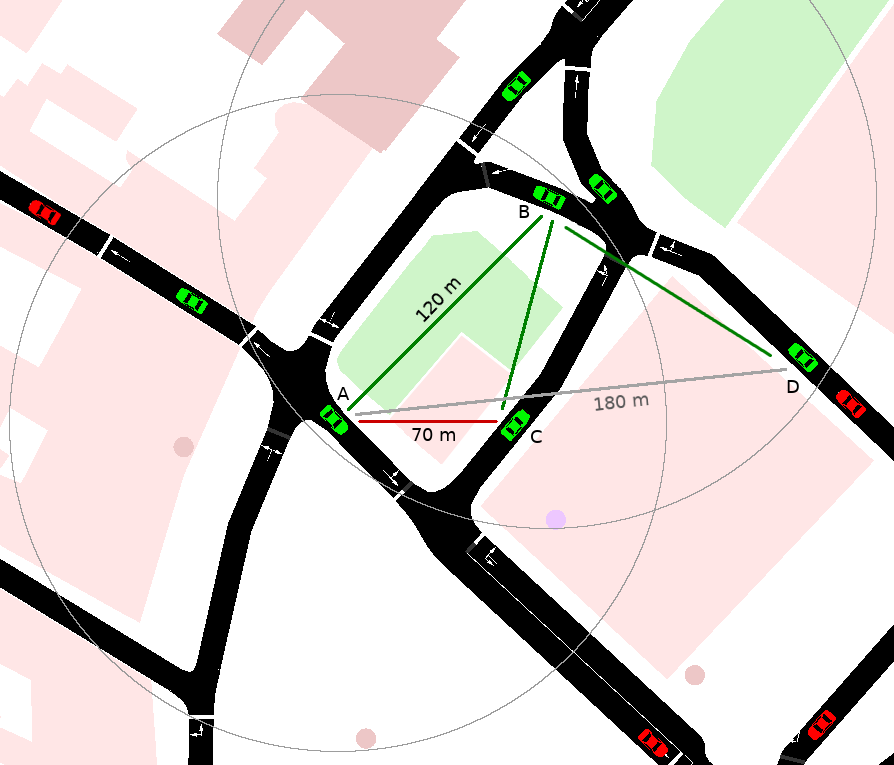
\includegraphics[width=\textwidth]{immagini/fb-2dpicc}
			\caption{Example of Fast-Broadcast in 2D scenario}
			\label{fig:fb-2d}
		\end{figure}
		
		
		
		For example, suppose that vehicle A is the origin of the Alert Message and B receives it, but C doesn't due to an obstacle in the line of sight. B computes origin-vehicle distance, $d(A, B)$, and origin-sender distance, $d(A, A)$, which in this case are respectively 120 and 0m. Since origin-vehicle is greater than origin-sender, B can forward the Alert Message.
		
		
		Now suppose that C receives the message from B. C computes origin-vehicle distance, $d(A, C)$, and origin-sender distance, $d(A, B)$, which amount to 70 and 120m respectively. Since the former is not greater than or equal to the latter, C is not a candidate for forwarding and suppresses the transmission.
		
		
		D receives the message from B as well. D is a good candidate for becoming the next forwarder since the origin-vehicle distance, which amounts to 180m, is greater than origin-sender distance, equal to 120m.
		
		However, the condition by which vehicles suppressed their transmission when the origin-sender distance was smaller than the origin-sender distance causes delivery problems in particular scenarios, reported in Appendix \ref{chapter:fbmod}. Hence, that condition has been dropped in the algorithm implemented in this work. Referring to the example in Figure \ref{fig:fb-2d}, this change makes vehicle C a forwarder candidate as well.
		
		Algorithm \ref{alg:hello-message-sending-2d}, \ref{alg:hello-message-receiving-2d}, \ref{alg:alert-message-generation-2d} and \ref{alg:alert-message-forwarding-2d} show the implementation for Fast-Broadcast for multiple dimensions (mainly 2D, but this version actually works also for 3D scenarios, for example scenarios with only drones or with drones and vehicles).
		
		\begin{algorithm}[H]
			\begin{algorithmic}[1]
				\ForEach{turn}
				\State sendingTime $\gets$ random(turnSize)
				\State wait(sendingTime)
				\If{$\neg$ (heardHelloMsg() $\lor$ heardCollision())}
				\State helloMsg.declaredMaxRange $\gets$ max(LMR, CMR)
				\State helloMsg.senderPosition $\gets$ retrievePosition()
				\State transmit(helloMsg)
				\EndIf
				\EndFor
			\end{algorithmic}
			\caption{Hello message sending procedure for 2D}
			\label{alg:hello-message-sending-2d}
		\end{algorithm}
		
		\begin{algorithm}[H]
			\begin{algorithmic}[1]
				\State myPosition $\gets$ retrievePosition()
				\State senderPosition $\gets$ helloMsg.senderPosition
				\State declaredMaxRange $\gets$ helloMsg.declaredMaxRange
				\State d $\gets$ distance(myPosition, senderPosition)
				\State CMR $\gets$ max(CMR, d, declaredMaxRange)
			\end{algorithmic}
			\caption{Hello message receiving procedure for 2D}
			\label{alg:hello-message-receiving-2d}
		\end{algorithm}
	
	
		\begin{algorithm}[H]
			\begin{algorithmic}[1]
				\State alertMsg.maxRange $\gets$ max(LMR, CMR)
				\State alertMsg.senderPosition $\gets$ retrievePosition()
				\State alertMsg.originPosition $\gets$ retrievePosition()
				\State transmit(alertMsg)
			\end{algorithmic}
			\caption{Alert Message generation procedure for 2D}
			\label{alg:alert-message-generation-2d}
		\end{algorithm}
	
		\begin{algorithm}[H]
			\begin{algorithmic}[1]
				\State cwnd $\gets$ computeCwnd()
				\State waitTime $\gets$ random(cwnd)
				\State wait(waitTime)
				\If{sameBroadcastHeardFromBack()}
				\State exit()
				\ElsIf{sameBroadcastHeardFromFront()}
				\State restartBroadcastProcedure()
				\Else 
				\State alertMsg.maxRange $\gets$ max(LMR, CMR)
				\State alertMsg.senderPosition $\gets$ retrievePosition()
				\State transmit(alertMsg)
				\EndIf 
			\end{algorithmic}
			\caption{Alert Message forwarding procedure for 2D}
			\label{alg:alert-message-forwarding-2d}
		\end{algorithm}
	
		\subsection{Hello Message Header Structure}
			The Hello Message header structure is represented in Figure \ref{fig:fbHelloHeader}.
			\begin{figure}[H]
				\centering
				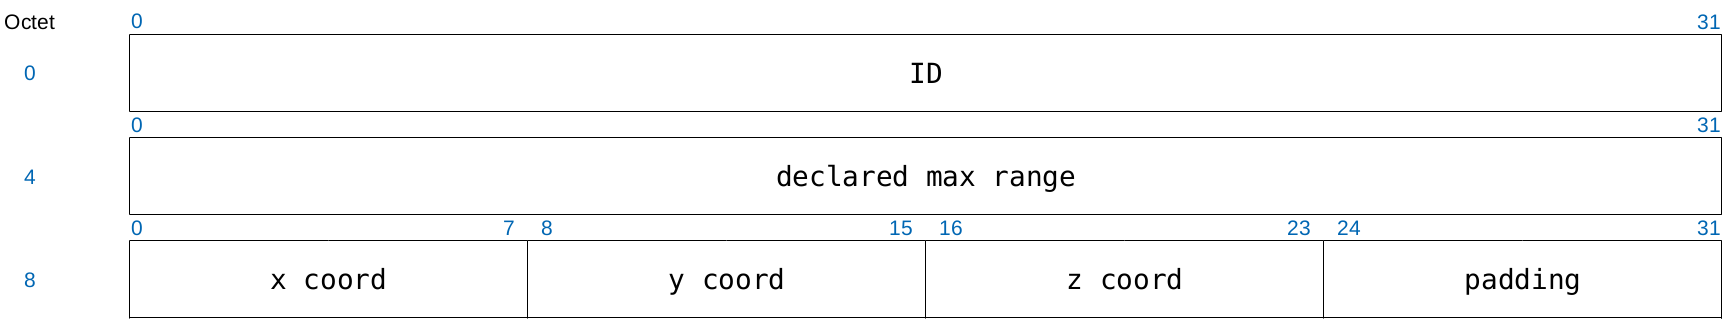
\includegraphics[width=\textwidth]{immagini/fbHelloHeader}
				\caption{Fast-Broadcast Hello Message header structure}
				\label{fig:fbHelloHeader}
			\end{figure}
			
			The fields contained in the Hello Message are the following:
			\begin{itemize}
				\item \textit{ID}: unique ID of the Hello Message's sender;
				\item \textit{declared max range}: maximum range detected by the vehicle during Estimation Phase;
				\item \textit{x coord}, \textit{y coord} and \textit{z coord}: coordinates of the Hello Message's sender.
			\end{itemize}
		
		\subsection{Alert Message Header Structure}
			The Alert Message header structure is represented in Figure \ref{fig:fbAlertHeader}.
			\begin{figure}[H]
				\centering
				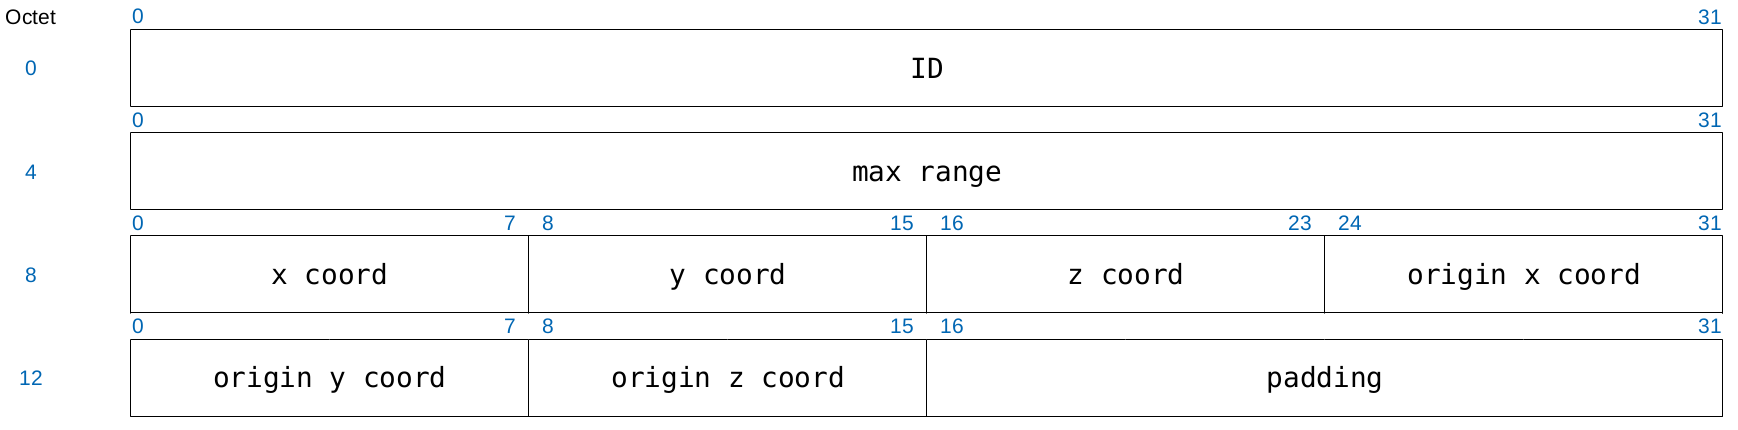
\includegraphics[width=\textwidth]{immagini/fbAlertHeader}
				\caption{Fast-Broadcast Alert Message header structure}
				\label{fig:fbAlertHeader}
			\end{figure}
		
		The fields contained in the Alert Message are the following:
		\begin{itemize}
			\item \textit{ID}: unique ID of the Alert Message's sender;
			\item \textit{max range}: maximum range detected by the vehicle during Estimation Phase;
			\item \textit{x coord}, \textit{y coord} and \textit{z coord}: coordinates of the Hello Message's sender;
			\item \textit{origin x}, \textit{origin y} and \textit{origin z coord}: coordinates where the Alert initially originated from.
		\end{itemize}
	
	\section{Smart Junction Fast-Broadcast (SJ-Fast-Broadcast)}
		\label{sj:fb}
		This work proposes an extension for Fast-Broadcast which keeps junctions into consideration in order to achieve a greater delivery ratio of Alert Messages. The idea comes from the following observation: whenever buildings block signal propagation across different roads, the message is relayed only through the road segments inside the forwarder's field of view. This causes the Alert Message propagation to spread:
		\begin{itemize}
			\item in one direction, if the forwarder is not inside a junction and the road segment is surrounded by buildings which block the signal;
			\item in three directions, whenever the forwarder lies inside a junction. 
		\end{itemize}
		Actually the signal travels respectively in two and four directions, but we are not considering the direction where the previous Alert Message is coming from (i.e., we are only considering forwarding towards previously uncovered areas in this analysis).
		Referring to Figure \ref{fig:fb-junction-0}, if the message is coming from the top and A and B forwards it, then only vehicles in the north-south road will be reached. Vehicles on the west-east road will be reached by the Alert Message at a later point, if the propagation circles back to them through another road, otherwise they will never be informed about the alert. If C is also forced to forward, then we have coverage across all road segments and the propagation can continue towards all directions. Figure \ref{fig:fb-junction-1} shows an example where SJ-Fast-Broadcast is employed and a greater coverage is achieved.
		
		\begin{figure}[H]
			\centering
			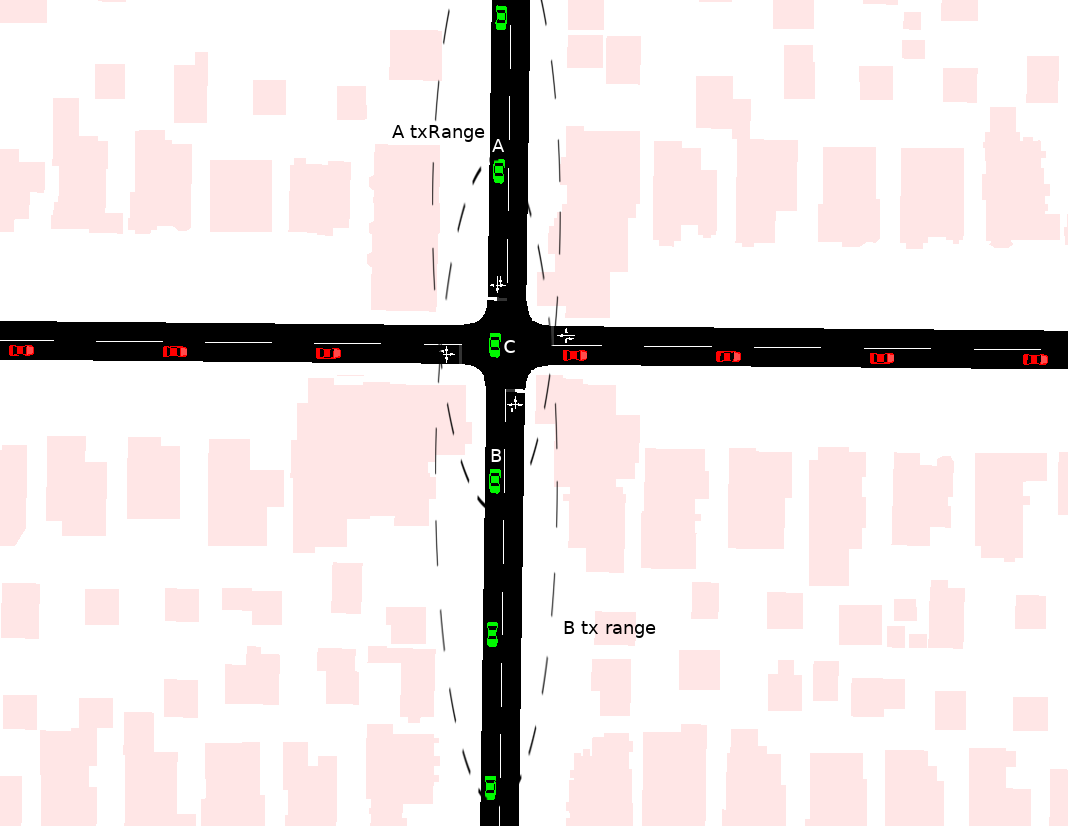
\includegraphics[width=\textwidth]{immagini/fb-junction-0}
			\caption{Regular Fast-Broadcast Alert Message propagation}
			\label{fig:fb-junction-0}
		\end{figure}
	
		\begin{figure}[H]
			\centering
			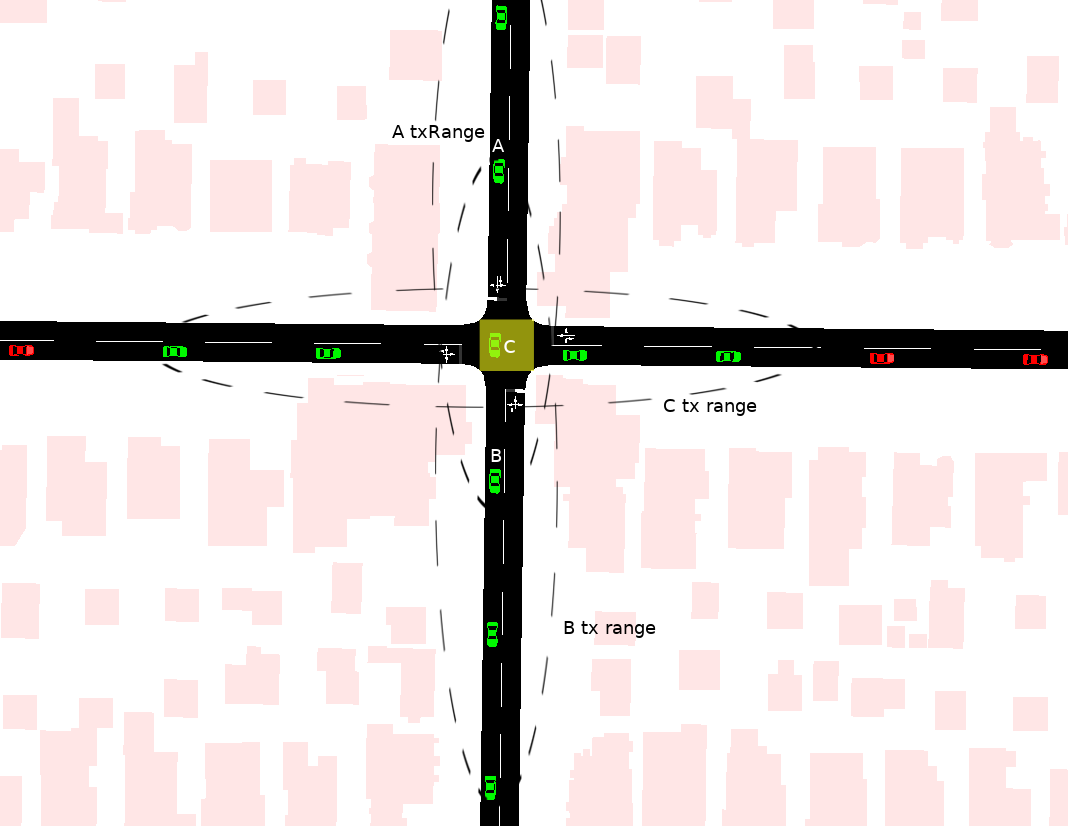
\includegraphics[width=\textwidth]{immagini/fb-junction-1}
			\caption{SJ-Fast-Broadcast Alert Message propagation}
			\label{fig:fb-junction-1}
		\end{figure}
		
		
		The proposed extension works by having nodes inside a junction participate in a second contention with all other vehicles inside the same junction. When the original timer calculated by Fast-Broadcast expires for one of the vehicles inside the junction, it forwards the message. All other vehicles inside the same junction suppress their transmission. This way the propagation can proceed in all directions, while the propagation in the normal direction can proceed without additional delays. Algorithm \ref{alg:sj-alert-message-generation} and \ref{alg:sj-alert-message-forwarding} show the code for SJ-Fast-Broadcast's Broadcast Phase. Estimation Phase's algorithms remain the same as Algorithm \ref{alg:hello-message-sending-2d} and \ref{alg:hello-message-receiving-2d}. Line 4 of Algorithm \ref{alg:sj-alert-message-forwarding} shows that a vehicle suppresses its transmission in one of the following two cases:
		\begin{itemize}
			\item if the vehicle has heard the same broadcast coming from the back and is not inside a junction;
			\item if the vehicle has heard the same broadcast coming from the back, is inside a junction with ID \textit{j} and the sender is also inside the same junction.
		\end{itemize}
		
		\begin{algorithm}[H]
			\begin{algorithmic}[1]
				\State alertMsg.maxRange $\gets$ max(LMR, CMR)
				\State alertMsg.senderPosition $\gets$ retrievePosition()
				\State alertMsg.originPosition $\gets$ retrievePosition()
				\State alertMsg.senderInJunction $\gets$ isSenderInJunction()
				\State alertMsg.junctionId $\gets$ getJunctionId()
				\State transmit(alertMsg)
			\end{algorithmic}
			\caption{SJ-Fast-Broadcast Alert Message generation procedure}
			\label{alg:sj-alert-message-generation}
		\end{algorithm}
		
		\begin{algorithm}[H]
			\begin{algorithmic}[1]
				\State cwnd $\gets$ computeCwnd()
				\State waitTime $\gets$ random(cwnd)
				\State wait(waitTime)
				\If{(sameBroadcastHeardFromBack() $\land$ vehicleNotInJunction()) $\lor$ (sameBroadcastHeardFromBack() $\land$ vehicleInJunction(j) $\land$ alertMsg.senderInJunction $\land$ alertMsg.junctionId == j)}
				\State exit()
				\ElsIf{sameBroadcastHeardFromFront()}
				\State restartBroadcastProcedure()
				\Else 
				\State alertMsg.maxRange $\gets$ max(LMBR, CMBR)
				\State alertMsg.senderPosition $\gets$ retrievePosition()
				\State transmit(alertMsg)
				\EndIf 
			\end{algorithmic}
			\caption{SJ-Fast-Broadcast Alert Message forwarding procedure}
			\label{alg:sj-alert-message-forwarding}
		\end{algorithm}
	
		\subsection{Alert Message Header Structure}
			The Hello Message header structure is the same as Figure \ref{fig:fbHelloHeader}, hence it is not reported here. The Alert Message header structure is represented in Figure \ref{fig:sj-fbAlertHeader}.
			
			\begin{figure}[H]
				\centering
				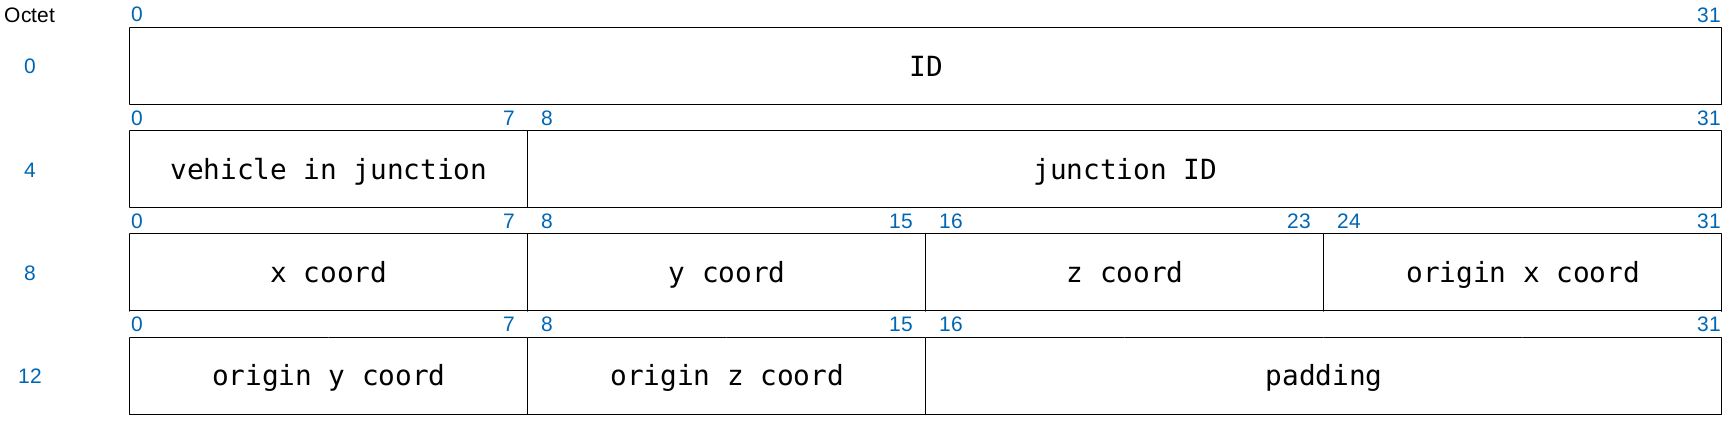
\includegraphics[width=\textwidth]{immagini/sj-fbAlertHeader}
				\caption{SJ-Fast-Broadcast Alert Message header structure}
				\label{fig:sj-fbAlertHeader}
			\end{figure}
			
			The additional fields are the following:
			\begin{itemize}
				\item  \textit{vehicle in junction}: whether the vehicle which is send this Alert Message is inside a junction;
				\item \textit{junction ID}: the ID of the junction the sender is inside.
			\end{itemize}